% Options for packages loaded elsewhere
\PassOptionsToPackage{unicode}{hyperref}
\PassOptionsToPackage{hyphens}{url}
%
\documentclass[
]{article}
\usepackage{amsmath,amssymb}
\usepackage{lmodern}
\usepackage{iftex}
\ifPDFTeX
  \usepackage[T1]{fontenc}
  \usepackage[utf8]{inputenc}
  \usepackage{textcomp} % provide euro and other symbols
\else % if luatex or xetex
  \usepackage{unicode-math}
  \defaultfontfeatures{Scale=MatchLowercase}
  \defaultfontfeatures[\rmfamily]{Ligatures=TeX,Scale=1}
\fi
% Use upquote if available, for straight quotes in verbatim environments
\IfFileExists{upquote.sty}{\usepackage{upquote}}{}
\IfFileExists{microtype.sty}{% use microtype if available
  \usepackage[]{microtype}
  \UseMicrotypeSet[protrusion]{basicmath} % disable protrusion for tt fonts
}{}
\makeatletter
\@ifundefined{KOMAClassName}{% if non-KOMA class
  \IfFileExists{parskip.sty}{%
    \usepackage{parskip}
  }{% else
    \setlength{\parindent}{0pt}
    \setlength{\parskip}{6pt plus 2pt minus 1pt}}
}{% if KOMA class
  \KOMAoptions{parskip=half}}
\makeatother
\usepackage{xcolor}
\usepackage[margin=1in]{geometry}
\usepackage{longtable,booktabs,array}
\usepackage{calc} % for calculating minipage widths
% Correct order of tables after \paragraph or \subparagraph
\usepackage{etoolbox}
\makeatletter
\patchcmd\longtable{\par}{\if@noskipsec\mbox{}\fi\par}{}{}
\makeatother
% Allow footnotes in longtable head/foot
\IfFileExists{footnotehyper.sty}{\usepackage{footnotehyper}}{\usepackage{footnote}}
\makesavenoteenv{longtable}
\usepackage{graphicx}
\makeatletter
\def\maxwidth{\ifdim\Gin@nat@width>\linewidth\linewidth\else\Gin@nat@width\fi}
\def\maxheight{\ifdim\Gin@nat@height>\textheight\textheight\else\Gin@nat@height\fi}
\makeatother
% Scale images if necessary, so that they will not overflow the page
% margins by default, and it is still possible to overwrite the defaults
% using explicit options in \includegraphics[width, height, ...]{}
\setkeys{Gin}{width=\maxwidth,height=\maxheight,keepaspectratio}
% Set default figure placement to htbp
\makeatletter
\def\fps@figure{htbp}
\makeatother
\setlength{\emergencystretch}{3em} % prevent overfull lines
\providecommand{\tightlist}{%
  \setlength{\itemsep}{0pt}\setlength{\parskip}{0pt}}
\setcounter{secnumdepth}{5}
\newlength{\cslhangindent}
\setlength{\cslhangindent}{1.5em}
\newlength{\csllabelwidth}
\setlength{\csllabelwidth}{3em}
\newlength{\cslentryspacingunit} % times entry-spacing
\setlength{\cslentryspacingunit}{\parskip}
\newenvironment{CSLReferences}[2] % #1 hanging-ident, #2 entry spacing
 {% don't indent paragraphs
  \setlength{\parindent}{0pt}
  % turn on hanging indent if param 1 is 1
  \ifodd #1
  \let\oldpar\par
  \def\par{\hangindent=\cslhangindent\oldpar}
  \fi
  % set entry spacing
  \setlength{\parskip}{#2\cslentryspacingunit}
 }%
 {}
\usepackage{calc}
\newcommand{\CSLBlock}[1]{#1\hfill\break}
\newcommand{\CSLLeftMargin}[1]{\parbox[t]{\csllabelwidth}{#1}}
\newcommand{\CSLRightInline}[1]{\parbox[t]{\linewidth - \csllabelwidth}{#1}\break}
\newcommand{\CSLIndent}[1]{\hspace{\cslhangindent}#1}
\newcommand{\beginappendix}{ \setcounter{table}{0} \renewcommand{\thetable}{A\arabic{table}} \setcounter{figure}{0} \renewcommand{\thefigure}{A\arabic{figure}} }
\usepackage[capposition=top]{floatrow}
\usepackage{placeins}
\usepackage{setspace}
\usepackage{dcolumn}
\usepackage{booktabs}
\usepackage{siunitx}
\usepackage{amsmath}
\usepackage{enumerate}
\usepackage[shortlabels]{enumitem}
\usepackage[hang,flushmargin]{footmisc}
\usepackage{booktabs}
\usepackage{longtable}
\usepackage{array}
\usepackage{multirow}
\usepackage{wrapfig}
\usepackage{float}
\usepackage{colortbl}
\usepackage{pdflscape}
\usepackage{tabu}
\usepackage{threeparttable}
\usepackage{threeparttablex}
\usepackage[normalem]{ulem}
\usepackage{makecell}
\usepackage{xcolor}
\ifLuaTeX
  \usepackage{selnolig}  % disable illegal ligatures
\fi
\IfFileExists{bookmark.sty}{\usepackage{bookmark}}{\usepackage{hyperref}}
\IfFileExists{xurl.sty}{\usepackage{xurl}}{} % add URL line breaks if available
\urlstyle{same} % disable monospaced font for URLs
\hypersetup{
  pdftitle={Pollution, agricultural productivity, and development: Evidence from coal in plants in India},
  pdfauthor={Joshua D. Merfeld},
  hidelinks,
  pdfcreator={LaTeX via pandoc}}

\title{Pollution, agricultural productivity, and development: Evidence from coal in plants in India\footnote{thanks to\ldots{}}}
\author{Joshua D. Merfeld\footnote{KDI School of Public Policy and Management and IZA; \href{mailto:merfeld@kdis.ac.kr}{\nolinkurl{merfeld@kdis.ac.kr}}}}
\date{2023-01-13}

\begin{document}
\maketitle
\begin{abstract}
\noindent The rapid increase in population in India from the 1990s through the 2010s led to the rapid construction of new coal power plants throughout the country. Using this roll-out combined with randdom changes in wind direction, I document negative effects of pollution from coal power plants on agricultural productivity throughout the country. Results suggest this decrease may be driven by a decline in labor allocation of the oldest half of my sample, though I cannot rule out direct effects of pollution on land productivity. These impacts spill over into aggregate economic growth, as well; nightlight growth is slower following years of higher exposure to pollution.\\
\strut \\
\textbf{\textit{Keywords}}: pollution, productivity, agriculture, labor, India\\
\textbf{\textit{JEL Codes}}: H40, I15, J22, O13, Q52, Q53
\end{abstract}

\newpage
\doublespacing

\hypertarget{introduction}{%
\section{Introduction}\label{introduction}}

From 1990 to 2010, India's population grew by more than 40 percent.\footnote{data.worldbank.org} This population growth led to a large increase in demand for power. While natural gas has become a popular alternative in much of the world, the Indian government met much of the increased demand through the construction of coal power plants. During those same two decades, power generation from all coal units of at least 30 megawatts increased by almost 140 percent, from 42.4 gigawatts to more than 100 gigawatts.\footnote{\url{https://globalenergymonitor.org/}} There are no doubt positive effects from this increase in power generation; for example, electricity may lead to economic and productivity growth (Dinkelman 2011; Kline and Moretti 2014; Rud 2012; Van de Walle et al. 2017), though electrification alone may not be a sufficient condition (Lee, Miguel, and Wolfram 2020).

These improvements do not come without downsides, however, especially when it comes to power derived from coal. Pollutants from coal contribute to climate change and the phase out of coal energy is therefore a major climate goal (IEA 2022). Emissions from the production and burning of coal are also directly harmful to health and the environment, including pollutants like sulfur dioxide, nitrogen oxides, and mercury, to name but a few.\footnote{\url{https://www.eia.gov/energyexplained/coal/coal-and-the-environment.php}} While the use of coal had been declining, recent events -- including Russia's invasion of Ukraine -- have led to an increase in the demand for coal.\footnote{\url{https://www.npr.org/2022/08/15/1117560560/a-rising-demand-for-coal-amidst-war-in-ukraine}}

In this paper, I study the effects of emissions from coal power plants on agricultural productivity, labor allocation, and economic growth in India. Previous work has suggested that there may be harmful direct effects of air pollution (Heck et al. 1982; Marshall et al. 1997) and water pollution (Reddy and Behera 2006) on agricultural productivity, including work showing that gold mines -- which release large amounts of pollutants into the surrounding environment -- lead to lower agricultural productivity in Ghana (Aragón and Rud 2016). This paper, however, tackles the broader case of coal plants, which are a leading source of power throughout the world. I show that pollution from these plants can lead to decreased agricultural productivity in the case of India.

I combine the roll out of coal plants in India with plausibly exogenous changes in wind direction -- in a similar spirit to (Deryugina et al. 2019) -- to measure the effects of pollution from coal plants on key development outcomes. I first locate the location of coal plants in India by year. Using village-level shapefiles, I identify all villages that are located within 30km of a coal plant at any timn during the sample period, which comprises the 1990s to the 2010s, with differences depending on data availability. I then download daily wind data and create an identifier for whether a village is located downwind from a coal plant on any given day, aggregating these daily values to different levels depending on the analysis.

After validating that wind direction is a strong predictor of particulate matter, I first document that the total number of days of being downwind from a coal power plant has a negative effect on overall agricultural productivity, using newly available estimates of India-wide agricultural (land) productivity. The within-village absolute deviation of wind exposure is around eight days, meaning that median changes in wind direction are responsible for fluctuations in agricultural productivity of around 2.4 percent, with changes of more than five percent from season to season being common. Using wind direction as an instrument for particulate matter, an increase of PM 2.5 by one microgram leads to an even larger decrease in agricultural productivity, at around 20 percent. This IV strategy is similar to that in Deryugina et al. (2019), though they use general ``high-pollution'' wind directions while I concentrate only on wind directions from the location of a coal power plant.

These effects are apparently concentrated in villages that do not experience the most extreme exposure to pollution; villages with higher maximum exposure experience effects only around 10 percent as large as villages with lower maximum exposure. Additional heterogeneity analysis shows that, despite the results with respect to the maximum, the effects are increasing in \emph{mean} exposure. I also show that the effects are largest in villages with the highest initial agricultural productivity and that pollution and rainfall shocks are compounding; higher exposure along with less rainfall increases the negative effect of either shock individually.

Robustness checks show that this effect is concentrated in the years after the construction of the power plant, which helps decrease concerns around endogeneity since, conditional on the village fixed effect and rainfall, windfall direction across years and seasons is exogenous. Additionally, leads for wind direction do not predict current agricultural productivity, again supporting the identifying assumptions.

While I am not able to explicitly test effects on land productivity, I look at how adults allocate labor over the last seven days using the National Sample Survey and creating a district-level exposure measure based on the timing of the survey for each household. An additional day of wind over the previous week decreases overall labor allocation by 0.027 days. However, all effects on labor allocation are driven by the older half of my sample; these adults see much large decreases in overall labor allocation, self employment, farm employment, and non-farm employment. This is suggestive evidence of productivity effects being driven by the health effects on individuals, though I am not able to rule out direct effects on land productivity with my data.

The final set of results explores whether there are impacts of pollution on aggregate economic development. Using nightlights, I show that lagged wind -- i.e.~pollution exposure in the prior year -- has a negative impact on economic development as proxied by nightlights. Going from the 25th percentile to the 75th percentile of wind exposure is synonymous with a decrease in the growth of nightlights within a village by around 0.7 percent. While this is a relatively small magnitude, it is worth noting that there are more than 100,000 villages in this sample. While the effect for a single village might be small, the overall, aggregate effect on growth is quite substantial.

This paper contributes to several strands of literature. First, we already have evidence of effects of pollution on different forms of labor activity. For example, general levels of pollution decrease productivity of call center works in China (Chang et al. 2019), lead people to perform worse on cognitive functions (Ebenstein, Lavy, and Roth 2016; Wen and Burke 2022), and also lead to lower levels of farm labor productivity in California, driven by changes in ozone concentration (Graff Zivin and Neidell 2012). Also in China, He, Liu, and Salvo (2019) find small but significant negative effects of pollution on manufacturing productivity, while Chen, Oliva, and Zhang (2022) show pollution leads to labor out migration. Perhaps relevant to my labor allocation results, Hanna and Oliva (2015) show that decreases in pollution lead to increases in labor allocation, while I show the same relationship among the oldest cohort. The paper most related to this one is Aragón and Rud (2016), who show that gold mines in Ghana have substantial negative impacts on agricultural productivity in the surrounding areas. This paper differs in two important ways. First, I explore effects of pollution from coal plants, which are much more ubiquitous than goald mines across the world. Second, I use a different identification strategy, relying on wind blowing pollution from coal plants.

I also contribute to the more general literature on the effects of pollution on health. Pollution has substantial negative effects on health in both developing and developed countries (Arceo, Hanna, and Oliva 2016) and we have known of these negative effects for many years (Brunekreef and Holgate 2002; Kampa and Castanas 2008; Pope III and Dockery 2006). Currie et al. (2014) review the literature on the health effects of pollution during adolescence; we have robust evidence of pollution exposure leading to increases in infant mortality, including in developing countries (Heft-Neal et al. 2018, 2019). Since these effects are often driven by heart and lung disease and asthma (Kampa and Castanas 2008), this my explain the labor allocation effects I identify in this paper.

The rest of the paper is organized as follows. I first discuss data and methodology. I break this section up into \autoref{data2}, which covers the multiple sources of data used in this paper; \autoref{identification}, which discusses the empirical strategy; and \autoref{validation}, which validates the wind direction variable using data on particulate matter. I present the main results in \autoref{results} before concluding in \autoref{conclusion}.

\hypertarget{data-and-methods}{%
\section{\texorpdfstring{Data and methods \label{data}}{Data and methods }}\label{data-and-methods}}

\hypertarget{data}{%
\subsection{\texorpdfstring{Data \label{data2}}{Data }}\label{data}}

The main goal of this paper is to examine whether exposure to exhaust from coal plants affects agricultural productivity, labor allocation, and economic growth. I use several sources of data, which I describe here and in Table \ref{tab:data} in the appendix.

The first set of data lists the location of coal plant across the globe. This data comes from Global Energy Monitor.\footnote{\url{https://globalenergymonitor.org/projects/global-coal-plant-tracker/}} and lists all units generating at least 30 megawatts of electricity. The data on coal plants includes the year of opening (and, if applicable, the year of retirement), the GPS (latitude/longitude) location of each plant, and the amount of power produced by the units at each plant. For this paper, I do not use the information on the capacity of the plant.

\begin{figure}
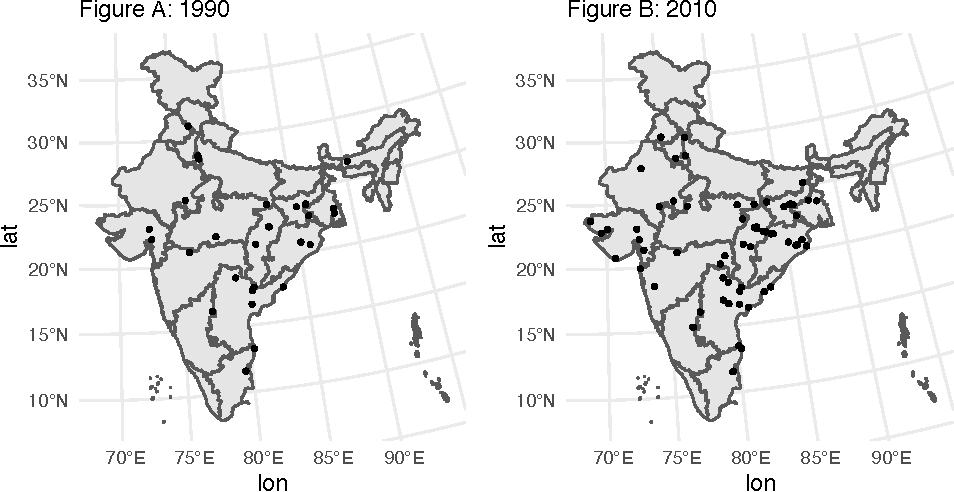
\includegraphics{draft_files/figure-latex/plants-1} \caption[Coal plants in India from 1990 to 2010]{Coal plants in India from 1990 to 2010}\label{fig:plants}\floatfoot*{Note: The top figure shows the location of coal plants in 1990. The bottom figure shows the location of coal plants in 2010.}
\end{figure}

Figure \ref{fig:plants} presents the location of coal plants in India for two specific years: 1990 and 2010. There is a clear increase in the prevalence of coal plants across the country over the two decades. Additionally, the overall capacity from coal plants increased from 42.4 gigawatts to 100.4 gigawats, an increase of 136.6 percent in just 20 years.

The second dataset includes agricultural productivity for both the monsoon and winter seasons, from 2002 to 2018. To match other data, I only use the data up to 2013. This data comes from Gangopadhyay et al. (2022) and estimates land productivity (i.e.~yield, in tons per hectare) for the major crops in India. They define the monsoon season as June to October and the winter season as November to March. I keep these definitions when matching across data below. This data is also publicly available from Nature's data-sharing website.\footnote{\url{https://springernature.figshare.com}}

The agricultural productivity data is available as raster files with a resolution of 500m. To aggregate this data up to a useful administrative unit, I use village-level shapefiles provided by Asher et al. (2021) and publicly available on the SHRUG platform.\footnote{\url{https://www.devdatalab.org/shrug_download/}} I aggregate the agricultural productivity data to the village level by extracting mean productivity for each feature in the shapefile. I do this separately for each season -- monsoon and winter -- and each year, from 2002 to 2013.

To measure exposure to pollution from coal plants, I first locate all village centroids located within 30km from a coal plant in a given year. I choose 30km due to previous research on the effects of (air) pollution (Aragón and Rud 2016; Bencko and Symon 1977; Li and Gibson 2014). I then calculate the direction from coal plants to all village centroids within that 30km radius. To define exposure, I then pull daily wind direction data from the National Center for Atmospheric Research.\footnote{\url{https://climatedataguide.ucar.edu/}} For each day, I document whether the wind is blowing towards each village centroid.\footnote{I define ``towards'' as within five degrees to help take into account that I am using village centroids, using the x and y components of wind speed.} I then temporally aggregate this daily data depending on the temporal definition of the corresponding outcome. For example, agricultural productivity is defined across five months (e.g.~the monsoon season is from June to October) so I count the total days a given village is exposed to wind during those five months.

\begin{figure}
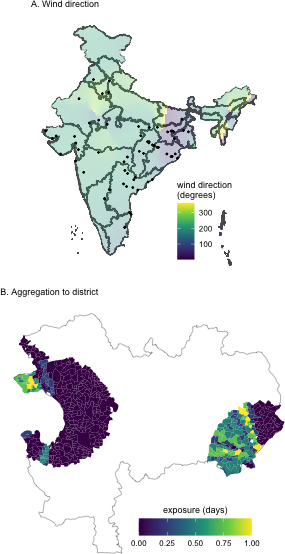
\includegraphics{draft_files/figure-latex/windexample-1} \caption[Wind direction and aggregation examples (2010-01-01)]{Wind direction and aggregation examples (2010-01-01)}\label{fig:windexample}\floatfoot*{Note: The left figure shows the average wind direction on January 1st, 2010. The points are the location of coal plants on that date. The right figure shows the distribution of pollution exposure in a specific district -- Kangra district in Himachal Pradesh -- on the same date.}
\end{figure}

The top panel in Figure \ref{fig:windexample} is an example wind direction raster. The raster shows wind direction for the entirety of India on January 1st, 2010, as well as the location of coal power plants on that date. The prevailing winds on the date differ across the country and, though not shown in the figure, across days. This means that the overall exposure for a given area to coal plant emissions changes across time. I also pull data on particulate matter to help validate this proxy for exposure. This data comes from Hammer et al. (2020) and I also aggregate this to the village using the same method detailed above.

To help understand some of the mechanisms driving the relationship between exposure to emissions and agricultural productivity, I also include household survey data. Unfortunately, I am not aware of any publicly available survey data that covers multiple years and has identifiers below the district level. For example, the ARIS-REDS data\footnote{\url{https://www.ncaer.org/project/additional-rural-incomes-survey-aris-rural-economic-demographic-survey-reds}} includes GPS identifiers for one year, but that only allows GPS matching for a total of two years: 1999 and 2007/2008. The DHS, on the other hand, only has district-level identifiers (except for the newest two waves) and is also not a labor survey. Instead, I use the National Sample Survey (NSS) from the Ministry of Statistics and Programme Implementation.

The NSS is a nationally representative survey that was conducted every couple of years until relatively recently. Many rounds of the NSS also included a module on employment that asked about labor allocation over the previous seven days. I use the 61st, 62nd, 64th, 66th, and 68th rounds of the NSS, all of which include the employment module. The publicly available data also includes the date of survey, which allows me to match pollution exposure to the exact day of the survey.

The biggest issue with using the NSS is that it includes only district-level identifiers. The main exposure variables, on the other hand, are defined at a lower level of aggregation, at the village. I choose to aggregate this village-level exposure to the district level as shown in the second panel of Figure \ref{fig:windexample}. I use the area overlap of the villages with the district to define a weighted average of exposure for the district at a given time. I calculate the area of overlap for each village and the district as well as the overall area of the district and use these variables to define weights for individual villages. Any part of the district that does not overlap with one of the villages -- the white area in Figure \ref{fig:windexample} -- does not have any exposure and, as such, receives a value of zero for exposure.

Finally, I use nightlights as a measure of economic growth (Henderson, Storeygard, and Weil 2012). I also take this data directly from SHRUG and Asher et al. (2021). This covers 1992 through 2013. Some of the older data may not be ideal (Gibson et al. 2021), but this is the only way to document changes in economic growth at a more disaggregated level and at a regular basis. Although satellite imagery is an attractive alternative (Burke et al. 2021), high-resolution satellite imagery does not go back to the early 1990s.

\hypertarget{identification}{%
\subsection{\texorpdfstring{Identification \label{identification}}{Identification }}\label{identification}}

To calculate the effects of exposure to pollution on different outcomes, I rely on fixed effects and the differential exposure driven by plausibly exogenous wind direction, conditional on total rainfall. The regession is of the form
\begin{gather} y_{it} = \alpha_{i} + \gamma_{t} + \beta wind_{it} + \delta rain_{it} + \varepsilon_{it}, \end{gather}
where \(y_{it}\) is outcome \(y\) for unit \(i\) at time \(t\), \(\alpha\) is a geographic fixed effects, \(\gamma_t\) is time fixed effects, \(wind_{it}\) is exposure to pollution -- defined using wind direction -- and \(rain_{it}\) is rainfall. Although I use \(i\) and \(t\) as subscripts for the fixed effects, note that these change depending on the unit of analysis and the outcome. I explicitly state the level of fixed effects in the tables and results below.

Identification relies on changes in wind direction across time for the same geographic units. In other words, conditional on the fixed effects and rainfall, I assume changes in wind direction are as good as random and uncorrelated with the outcome -- e.g.~agricultural productivity -- except through exposure to pollution. One major threat to identification is that the building of a coal plant could lead to a spurious correlation between the exposure variable and the outcome. Specifically, since exposure is defined as zero prior to the building of a coal plant, the exposure variable itself might be endogenous even though wind direction is not. To help allay these concerns, I estimate additional regressions restricting the sample to only time periods after which a given location has a coal plant. I also present results using leads to show that future wind direction does not seem to predict current outcomes.

\hypertarget{an-example-validating-wind-direction}{%
\subsection{\texorpdfstring{An example: validating wind direction \label{validation}}{An example: validating wind direction }}\label{an-example-validating-wind-direction}}

Before moving on to the main results, it is worth taking the time to better understand the fixed effects strategy with an example. Consider the data used for the regressions presented in Table \ref{tab:pollutiontable}. The outcome variable is particulate matter -- specifically, \(\mathrm{PM_{2.5}}\), which is particulate matter no larger than 2.5 micrometers in diameter -- which comes from Hammer et al. (2020). \(\mathrm{PM_{2.5}}\) is one of the harmful byproducts from coal plants, along with sulfur dioxide, different types of nitrogen oxides, and mercury.\footnote{\url{https://www.epa.gov/airmarkets/power-plants-and-neighboring-communities}} This data is available at the monthly level, so in Table \ref{tab:pollutiontable}, I aggregate wind exposure to the monthly level, as well.

\begin{table}

\caption{\label{tab:pollutiontable}Wind direction and particulate matter}
\centering
\begin{threeparttable}
\begin{tabular}[t]{>{\raggedright\arraybackslash}p{4cm}>{\centering\arraybackslash}p{2cm}>{\centering\arraybackslash}p{2cm}>{\centering\arraybackslash}p{2cm}>{\centering\arraybackslash}p{2cm}}
\toprule
\multicolumn{1}{c}{ } & \multicolumn{2}{c}{1998-2015} & \multicolumn{2}{c}{2002-2013} \\
\cmidrule(l{3pt}r{3pt}){2-3} \cmidrule(l{3pt}r{3pt}){4-5}
  & (1) & (2) & (3) & (4)\\
\midrule
wind & 0.045*** & 0.014*** & 0.063*** & 0.015***\\
 & (0.004) & (0.001) & (0.005) & (0.002)\\
\textbf{fixed effects:} & \textbf{} & \textbf{} & \textbf{} & \textbf{}\\
village & Yes & Yes & Yes & Yes\\
month & Yes & No & Yes & No\\
district-month & No & Yes & No & Yes\\
\midrule
observations & 22,345,092 & 22,345,092 & 14,896,728 & 14,896,728\\
\bottomrule
\end{tabular}
\begin{tablenotes}
\item Note: Standard errors are in parentheses and are clustered at the village level.
\item * p<0.10 ** p<0.05 *** p<0.01
\end{tablenotes}
\end{threeparttable}
\end{table}

Both the particulate matter data and the wind data is at the village level, which means the regressions in Table \ref{tab:pollutiontable} are at the village level. As such, the geographic fixed effects are village fixed effects and the temporal fixed effects are month fixed effects. Since the exposure variable is at the village level and we follow villages over time, the standard errors are also clustered at the village level.

In addition to serving as an example, Table \ref{tab:pollutiontable} also helps validate the use of wind direction as a proxy for exposure to pollution. The first two columns include all available years of data while the last two columns restrict estimation only to the years for which the agricultural productivity regressions are estimated. Across all four columns, the story is the same: when the wind is blowing in the direction of a village from a coal plant within 30 kilometers, estimated \(\mathrm{PM_{2.5}}\) is substantially higher. The regressions indicate that one additional day of wind in the direction of the village increases mean \(\mathrm{PM_{2.5}}\) for the month by between 0.014 and 0.045 \(\mathrm{\mu g/m^3}\).

To put these numbers into perspective, the World Health Organization's updated guidelines are that average annual exposure should not exceed 15 \(\mathrm{\mu g/m^3}\). For the month, an increase at the midpoint of the estimated range is equal to an increase of 0.2 percent of the maximum recommended mean concentration from the WHO. This is just a single day of wind in the direction of a village. Since this includes all villages located within 30km of a coal plant, this is evidence that wind direction can have serious repercussions on the health of hundreds of millions of people in India.

\hypertarget{results}{%
\section{\texorpdfstring{Results \label{results}}{Results }}\label{results}}

This section presents the main results of this paper. I present three sets of results: one set looking at agricultural productivity, another looking at labor allocation, and a final set looking at nightlights, which are a proxy for economic development. I go through each of these in turn.

\hypertarget{agricultural-productivity}{%
\subsection{Agricultural productivity}\label{agricultural-productivity}}

I first present results for agricultural productivity. The outcome of all the regressions in this section is the log of agricultural land productivity, which is defined as tons per hectare. The first set of results are in Table \ref{tab:yieldtable}. The unit of analysis is the year season -- from 2002 to 2013 -- the geographic fixed effect is the village-season, and the temporal fixed effect is the year. The exposure variable is defined for the entire season. Since Gangopadhyay et al. (2022) define both the monsoon (kharif) season and the winter (rabi) season as five months long, I do as well. This implies that the exposure variable ranges from zero to slightly more than 150.

The first column presents the most simple results, with only the wind exposure variable and the fixed effects. The second column adds a rainfall variable -- defined as the total rainfall in the season -- the addition of which is motivated by the fact that changes in wind direction could be correlated with changes in weather. However, the coefficient on the wind exposure variable is completely unchanged by the addition of rainfall, indicating that weather may not be as worrisome of a confounder as thought.

Column three adds district-by-year-by-season fixed effects as an additional robustness checks. This addition decreases the magnitude of the exposure variable but it remains negative and significant. However, part of this may be due to the fact that the new fixed effects soak up much of the variation in the exposure variable, as shown in Figure \ref{fig:windexample}. The last two columns separate the effects into the monsoon season and the winter season, but the overall effect is roughly similar, though rainfall has a larger effect in the monsoon season than the winter season, which is unsurprising.

\begin{table}

\caption{\label{tab:yieldtable}Wind direction and agricultural productivity}
\centering
\begin{threeparttable}
\begin{tabular}[t]{>{\raggedright\arraybackslash}p{3cm}>{\centering\arraybackslash}p{2cm}>{\centering\arraybackslash}p{2cm}>{\centering\arraybackslash}p{2cm}>{\centering\arraybackslash}p{2cm}>{\centering\arraybackslash}p{2cm}}
\toprule
\multicolumn{1}{c}{ } & \multicolumn{3}{c}{all} & \multicolumn{1}{c}{monsoon} & \multicolumn{1}{c}{winter} \\
\cmidrule(l{3pt}r{3pt}){2-4} \cmidrule(l{3pt}r{3pt}){5-5} \cmidrule(l{3pt}r{3pt}){6-6}
  & (1) & (2) & (3) & (4) & (5)\\
\midrule
wind & -0.003*** & -0.003*** & -0.0007*** & -0.002*** & -0.003***\\
 & (0.0002) & (0.0002) & (9.21e-5) & (0.0002) & (0.0003)\\
rain (z) &  & 0.029*** & 0.009*** & 0.082*** & 0.016***\\
 &  & (0.0004) & (0.001) & (0.002) & (0.0004)\\
\textbf{fixed effects:} & \textbf{} & \textbf{} & \textbf{} & \textbf{} & \textbf{}\\
village-season & Yes & Yes & Yes & No & No\\
year & Yes & Yes & No & Yes & Yes\\
district-year-season & No & No & Yes & No & No\\
village & No & No & No & Yes & Yes\\
\midrule
observations & 2,391,533 & 2,375,337 & 2,375,337 & 1,259,123 & 1,116,214\\
\bottomrule
\end{tabular}
\begin{tablenotes}
\item Note: Standard errors are in parentheses and are clustered at the village level.
\item * p<0.10 ** p<0.05 *** p<0.01
\end{tablenotes}
\end{threeparttable}
\end{table}

To put the size of the coefficient in context, it is worth digging a little deeper into the exposure variable. The mean within-village absolute deviation in wind exposure is approximately 8.06 days, meaning that the average change in agricultural productivity from year-to-year due to nothing but changes in wind patterns carrying particulate matter is around 2.4 percent relative to the mean. This implies that swings in agricultural productivity -- due to wind direction -- of more than five percent are probably quite common, since the absolute deviation includes deviations below and above the mean.

\begin{table}

\caption{\label{tab:yieldtabletwo}Pollution and agricultural productivity, IV estimates}
\centering
\begin{threeparttable}
\begin{tabular}[t]{>{\raggedright\arraybackslash}p{3.5cm}>{\centering\arraybackslash}p{2cm}>{\centering\arraybackslash}p{2cm}>{\centering\arraybackslash}p{2cm}>{\centering\arraybackslash}p{2cm}>{\centering\arraybackslash}p{2cm}}
\toprule
\multicolumn{1}{c}{ } & \multicolumn{3}{c}{all} & \multicolumn{1}{c}{monsoon} & \multicolumn{1}{c}{winter} \\
\cmidrule(l{3pt}r{3pt}){2-4} \cmidrule(l{3pt}r{3pt}){5-5} \cmidrule(l{3pt}r{3pt}){6-6}
  & (1) & (2) & (3) & (4) & (5)\\
\midrule
particulate matter & -0.021*** & -0.020*** & -0.033*** & -0.013*** & -0.024***\\
(PM 2.5) & (0.001) & (0.002) & (0.005) & (0.001) & (0.003)\\
rain (z) &  & 0.004** & 0.002 & 0.086*** & -0.016***\\
 &  & (0.002) & (0.002) & (0.002) & (0.004)\\
\textbf{fixed effects:} & \textbf{} & \textbf{} & \textbf{} & \textbf{} & \textbf{}\\
village-season & Yes & Yes & Yes & No & No\\
year & Yes & Yes & No & Yes & Yes\\
district-year-season & No & No & Yes & No & No\\
village & No & No & No & Yes & Yes\\
\midrule
observations & 2,391,533 & 2,375,337 & 2,375,337 & 1,259,123 & 1,116,214\\
\midrule
\textbf{first stage:} & \textbf{} & \textbf{} & \textbf{} & \textbf{} & \textbf{}\\
wind & 0.143*** & 0.126*** & 0.022*** & 0.155*** & 0.105***\\
 & (0.003) & (0.003) & (0.002) & (0.003) & (0.004)\\
rain (z) &  & -1.23*** & -0.235*** & 0.301*** & -1.36***\\
 &  & (0.010) & (0.018) & (0.015) & (0.009)\\
\bottomrule
\end{tabular}
\begin{tablenotes}
\item Note: Standard errors are in parentheses and are clustered at the village level.
\item * p<0.10 ** p<0.05 *** p<0.01
\end{tablenotes}
\end{threeparttable}
\end{table}

If you believe that wind direction is exogenous and, conditional on the fixed effects and rainfall, only affects agricultural productivity through pollution -- which seems reasonable since it is hard to imagine what other variables it might affect -- then it is a valid instrument for
pollution. While I opt to present the reduced form results for the rest of this paper, it is nonetheless an interesting exercise to also use wind direction as an instrument for pollution, which I measure using estimated \(\mathrm{PM_{2.5}}\) from Hammer et al. (2020).

The IV results appear in Table \ref{tab:yieldtabletwo}, with the second-stage results in the top panel and the first-stage results in the bottom panel. The first-stage results make clear how strong of an instrument wind is; also note that the coefficients are quite different from those in Table \ref{tab:pollutiontable} because the unit of analysis in Table \ref{tab:yieldtabletwo} is the season, while in Table \ref{tab:pollutiontable} the unit of analysis is the month.

The second-stage results indicate that \(\mathrm{PM_{2.5}}\) is a very strong predictor of agricultural productivity. The smallest coefficient -- that for the monsoon season in column (4) -- and the mean absolute deviation for \(\mathrm{PM_{2.5}}\) point to a change in agricultural productivity of around 23 percent.

\begin{table}

\caption{\label{tab:yieldtablehet}Heterogeneity in the effects of pollution on productivity}
\centering
\begin{threeparttable}
\begin{tabular}[t]{>{\raggedright\arraybackslash}p{4cm}>{\centering\arraybackslash}p{2cm}>{\centering\arraybackslash}p{2cm}>{\centering\arraybackslash}p{2cm}>{\centering\arraybackslash}p{2cm}>{\centering\arraybackslash}p{2cm}}
\toprule
\multicolumn{1}{c}{ } & \multicolumn{1}{c}{>p(50)} & \multicolumn{1}{c}{<=p(50)} & \multicolumn{3}{c}{all} \\
\cmidrule(l{3pt}r{3pt}){2-2} \cmidrule(l{3pt}r{3pt}){3-3} \cmidrule(l{3pt}r{3pt}){4-6}
  & (1) & (2) & (3) & (4) & (5)\\
\midrule
wind & -0.003*** & -0.032*** & -0.004*** & 0.0004 & -0.0001\\
 & (0.0002) & (0.002) & (0.0003) & (0.0005) & (0.001)\\
rain (z) & 0.031*** & 0.030*** & 0.029*** & 0.029*** & 0.029***\\
 & (0.0006) & (0.0005) & (0.0004) & (0.0004) & (0.0004)\\
wind x rain &  &  & 0.0005*** &  & \\
 &  &  & (6.67e-5) &  & \\
wind squared &  &  &  & -0.0002*** & \\
 &  &  &  & (3.54e-5) & \\
wind x starting yield &  &  &  &  & -0.001**\\
 &  &  &  &  & (0.0006)\\
\textbf{fixed effects:} & \textbf{} & \textbf{} & \textbf{} & \textbf{} & \textbf{}\\
village-season & Yes & Yes & Yes & Yes & Yes\\
year & Yes & Yes & Yes & Yes & Yes\\
\midrule
observations & 1,115,694 & 1,259,643 & 2,375,337 & 2,375,337 & 2,371,364\\
\bottomrule
\end{tabular}
\begin{tablenotes}
\item Note: Standard errors are in parentheses and are clustered at the village level.
\item * p<0.10 ** p<0.05 *** p<0.01
\end{tablenotes}
\end{threeparttable}
\end{table}

Having established that exposure to pollution has a negative effect on agricultural productivity, I now move to heterogeneity in these effects. Table \ref{tab:yieldtablehet} presents four different analyses: effects of exposure by maximum exposure, multiplicative effects of shocks, the possibility of non-linearities, and the differential effects of exposure based on initial agricultural productivity.

The first two columns split the sample based on average exposure; villages with maximum exposure above the median are included in column (1) while those below the median are in column (2). Interestingly, the largest effects are seen on villages in the lower half of the distribution. Apparently, smaller maximum effects lead to larger overall effects of pollution exposure on agricultural productivity. In other words, it is not the places where wind is most likely to blow from a coal plant that experience the largest decrease in productivity in response to an additional day of wind-driven pollution.

Column three looks add the possible multiplicative effects of rainfall shocks and pollution shocks on agricultural productivity. In previous tables, rainfall always entered the regression positively -- as we would expect -- indicating that higher rainfall in a given season leads to higher agricultural productivity. However, an interesting question is whether rainfall and pollution shocks might interact. The positive coefficient on the interaction term between days of wind and rainfall during the agricultural season indicates that there is a multiplicative effect of shocks; when wind days are higher (bad) and rainfall is lower (bad), the overall negative effects are even worse than when just one shock happens. Considering that climate change is leading to more variable rainfall and more negative rainfall shocks, these results are potentially worrisome, especially for smallholders.

Column four adds a quadratic in wind to see if the negative effects of pollution on agricultural productivity are increase or decreasing in wind. In column four, the coefficient on the linear term is 0.0004 while the coefficient on the quadratic term is -0.0002, meaning that the effect of wind is decreasing for any days of wind over two. The negative coefficient also indicates that this negative effect is consistently decreasing, meaning the effect gets worse as average wind days gets higher. Note that this is somewhat different from the regressions in the first two columns, which split the sample by the \emph{maximum} days of wind observed in the sample, not the mean.

In the final column I add to the regression an interaction between wind and initial agricultural productivity (defined in 2002, the first year observed in the productivity data). The linear term drops out of the regression since it is invariant within villages, leaving just the interaction term. The negative coefficient on the interaction term of -0.001 indicates that the effect of wind is more negative in areas where agricultural productivity is higher. Note that agricultural productivity is defined in logs, so this can be interpreted as a percentage effect, not a level effect. Apparently, wind-driven pollution is particularly detrimental to agricultural productivity in the most productive places.

\hypertarget{robustness-checks}{%
\subsection{Robustness checks}\label{robustness-checks}}

I present two separate robustness checks in the appendix. The first set of analyses attempts to separate the possible endogenous location of coal plants from outcomes. Specifically, prior to the opening of a new coal plant in an area, all villages receive a zero for wind. This means that, even if wind direction is exogenous, the opening of the coal plant could lead to correlations between the error term and the wind variable.

Although the results with district-year-season help mitigate this concern, Table \ref{tab:yieldtablepostplant} in the appendix checks this possibility in a different way. Specifically, I restrict the sample to only village-years \emph{after} the introduction of a coal plant. This drops any pre-plant-opening observations -- all of which are mechanically zeros for wind -- to prevent endogeneity due to the opening. The coefficients in Table \ref{tab:yieldtablepostplant} show that the overall effects are essentially unchanged, with just a small change in coefficient magnitude (driven mostly by rounding).

The second robustness check includes leads for wind to see if they predict current year productivity. I present these results in \ref{tab:yieldtableleads}. The second column includes district-year-season fixed effects, while the first does not. The results make clear the importance of including trends or district-year fixed effects. In the first column, leads seem to predict productivity. However, this relationship disappears in the second column, indicating that the previous results with district-year fixed effects are likely the most reliable.

\hypertarget{labor-allocation}{%
\subsection{Labor allocation}\label{labor-allocation}}

The previous set of results show a consistent negative effect of wind-driven pollution on agricultural productivity. A key question is the mechanism through which this happens; is this driven by changes in labor allocation/productivity or by changes in land productivity? While I cannot definitely prove the mechanism, I can shed some light on possibilities by looking at labor allocation decisions. Since these shocks generally happen after initial planting decisions, it seems unlikely that changes in land \emph{allocation} could drive the results.

Table \ref{tab:labortable} presents results for labor allocation over the last seven days using the National Sample Survey and the methodology described above. Since the labor recall is for seven days, labor allocation ranges from zero to seven, as does the wind variable. Recall that the data is at the district level, not the village level. However, it is also more temporally disaggregated, with rolling interviews throughout the year-long survey. Figure \ref{fig:laborplot} in the appendix shows this temporal distribution across the five waves of the survey.

There are some interesting results in Table \ref{tab:labortable}. The first two columns show a marginally significant decrease in overall labor allocation (where ``labor'' is defined as non-domestic self and wage employment). The third and fourth columns show that this overall decrease is predominantly from wage employment, not self employment. An additional day of wind over the last seven decreases wage employment by 0.034 days in the district. Mean wage employment is 1.458 days, meaning one day of wind decreases wage employment by 2.3 percent of the mean. Since much of the district is not covered by ``treated'' villages, this is actually a rather substantive effect on the villages involved.

The last two columns split the effects by sector, into farm and non-farm employment. Although agricultural (land) productivity decreases when wind blows in the direction of villages, overall labor allocation to farm labor actually goes \emph{up}, by around 4.5 percent of the mean of 0.784 days. Non-farm labor, on the other hand, goes down, by around 2.4 percent of the mean of 2.527 days.

There are two possible explanations for this pattern of results. First, it could be that land productivity goes down, leading farmers to increase their farm labor allocation in an attempt to compensate for the decreased productivity. A second possibility is that pollution does not affect land productivity at all, at least not directly. In this scenario, the worsening air quality could lead to decreased labor productivity, meaning that ``effective labor'' essentially decreases when pollution is higher. Unfortunately, I am not able to disentangle these two possiblities with the data available.

Table \ref{tab:labortablemonsoon} and Table \ref{tab:labortablewinter} in the appendix disaggregate these effects into the monsoon and winter seasons. Apparently, the entirety of the effect is driven by changes in labor allocation during the monsoon season. The dynamics across seasons apparently lead to large differences in the effects of pollution on labor allocation.

\begin{table}

\caption{\label{tab:labortable}Wind direction and labor allocation}
\centering
\begin{threeparttable}
\begin{tabular}[t]{>{\raggedright\arraybackslash}p{3cm}>{\centering\arraybackslash}p{1.5cm}>{\centering\arraybackslash}p{1.5cm}>{\centering\arraybackslash}p{1.5cm}>{\centering\arraybackslash}p{1.5cm}>{\centering\arraybackslash}p{1.5cm}>{\centering\arraybackslash}p{1.5cm}}
\toprule
  & all & all & self & wage & farm & non-farm\\
\midrule
wind & -0.021 & -0.027* & 0.008 & -0.034** & 0.035* & -0.061**\\
 & (0.015) & (0.015) & (0.017) & (0.016) & (0.019) & (0.025)\\
controls & No & Yes & Yes & Yes & Yes & Yes\\
\textbf{fixed effects:} & \textbf{} & \textbf{} & \textbf{} & \textbf{} & \textbf{} & \textbf{}\\
district & Yes & Yes & Yes & Yes & Yes & Yes\\
year & Yes & Yes & Yes & Yes & Yes & Yes\\
\textbf{varying slopes:} & \textbf{} & \textbf{} & \textbf{} & \textbf{} & \textbf{} & \textbf{}\\
year (by district) & Yes & Yes & Yes & Yes & Yes & Yes\\
\midrule
observations & 899,045 & 898,856 & 898,856 & 898,856 & 898,856 & 898,856\\
\bottomrule
\end{tabular}
\begin{tablenotes}
\item Note: Standard errors are in parentheses and are clustered at the district level. Control variables include female, age, age squared, and (years of) education.
\item * p<0.10 ** p<0.05 *** p<0.01
\end{tablenotes}
\end{threeparttable}
\end{table}

Previous research has shown larger effects of pollution on the health of the oldest (Deryugina et al. 2019). The labor sample includes all adults between 15 and 60 years of age. To look at heterogeneity by age, I present an additional set of results interacting the wind variable with an indicator for whether an individual is over 37 years of age.\footnote{This splits the sample into two equal bins of age: those who are 15-37 and those who are 38-60.} These results are in Table \ref{tab:labortableold}, which otherwise presents the same specifications in the last five columns as \ref{tab:labortable}.

\begin{table}

\caption{\label{tab:labortableold}Wind direction and labor allocation, heterogeneity by age}
\centering
\begin{threeparttable}
\begin{tabular}[t]{>{\raggedright\arraybackslash}p{4cm}>{\centering\arraybackslash}p{1.5cm}>{\centering\arraybackslash}p{1.5cm}>{\centering\arraybackslash}p{1.5cm}>{\centering\arraybackslash}p{1.5cm}>{\centering\arraybackslash}p{1.5cm}}
\toprule
  & all & self & wage & farm & non-farm\\
\midrule
wind & 0.061*** & 0.096*** & -0.034 & 0.068*** & -0.006\\
 & (0.023) & (0.022) & (0.024) & (0.020) & (0.030)\\
wind times age>=38 & -0.207*** & -0.207*** & -0.0001 & -0.078*** & -0.129***\\
 & (0.037) & (0.033) & (0.040) & (0.020) & (0.030)\\
controls & Yes & Yes & Yes & Yes & Yes\\
\textbf{fixed effects:} & \textbf{} & \textbf{} & \textbf{} & \textbf{} & \textbf{}\\
district & Yes & Yes & Yes & Yes & Yes\\
year & Yes & Yes & Yes & Yes & Yes\\
\textbf{varying slopes:} & \textbf{} & \textbf{} & \textbf{} & \textbf{} & \textbf{}\\
year (by district) & Yes & Yes & Yes & Yes & Yes\\
\midrule
observations & 898,856 & 898,856 & 898,856 & 898,856 & 898,856\\
\bottomrule
\end{tabular}
\begin{tablenotes}
\item Note: Standard errors are in parentheses and are clustered at the district level. Control variables include female, age, age squared, and (years of) education.
\item * p<0.10 ** p<0.05 *** p<0.01
\end{tablenotes}
\end{threeparttable}
\end{table}

Table \ref{tab:labortableold} presents a very clear set of results: the effects are always larger (more negative) for older adults. Particularly interestingly, we now see that the mean-zero effect on self employment in the previous table is driven by two stark contrasts: a large increase for the younger group and a large decrease for the older group. For the youngest group, this increase appears in farm labor, indicating likely increases in farm self-employment. The oldest, on the other hand, have large decreases in both farm and non-farm labor, with larger decreases in the latter.

While speculative, one possible explanation for this pattern is a decrease in labor productivity. While the youngest may be able to readjust and increase their overall self-employment labor allocation, perhaps the oldest cannot due to, for example, health effects of pollution, which are well documented (Bentayeb et al. 2012; Pope 3rd 2000).\footnote{Much of the literature also suggests the youngest are at significant risk of mortality and morbidities. However, given my focus on labor allocation, I only discuss older adults here.}

\hypertarget{nightlights}{%
\subsection{Nightlights}\label{nightlights}}

Pollution leads to lower agricultural productivity as well as changes in labor allocation. This leads to an obvious question: might higher levels of pollution also directly affect economic growth? To explore this question, I look at changes in nightlights relative to changes in pollution. It seems reasonable to think that pollution might affect nightlights with a lag, so I include the lag of pollution rather than contemporaneous pollution.

\begin{table}

\caption{\label{tab:ntltable}Wind direction and nightlight growth}
\centering
\begin{threeparttable}
\begin{tabular}[t]{>{\raggedright\arraybackslash}p{3cm}>{\centering\arraybackslash}p{2cm}>{\centering\arraybackslash}p{2cm}}
\toprule
  & (1) & (2)\\
\midrule
wind (lagged) & -0.080*** & -0.083***\\
 & (0.015) & (0.015)\\
rain (z, lagged) &  & -0.035***\\
 &  & (0.002)\\
\textbf{fixed effects:} & \textbf{} & \textbf{}\\
village & Yes & Yes\\
year & Yes & Yes\\
\textbf{varying slopes:} & \textbf{} & \textbf{}\\
year (by village) & Yes & Yes\\
\midrule
observations & 2,146,715 & 2,146,715\\
\bottomrule
\end{tabular}
\begin{tablenotes}
\item Note: Standard errors are in parentheses and are clustered at the village level.
\item * p<0.10 ** p<0.05 *** p<0.01
\end{tablenotes}
\end{threeparttable}
\end{table}

I present these results in Table \ref{tab:ntltable}. To help simplify the coefficients, I recode wind to be the proportion of days in the year that a given village experiences wind in their direction, from a coal plant. Mean wind in this new specification is 0.066, indicating that a village in the sample experiences wind in its direction on around 6.6 percent of days, or 24 days of the year.

We see a strong, negative relationship between pollution (lagged wind) and nightlights. Going from the 25th percentile to the 75th percentile of wind exposure is synonymous with a decrease in the growth of nightlights within a village by around 0.7 percent. While this is a relatively small magnitude, it is worth noting that there are more than 100,000 villages in this sample. While the effect for a single village might be small, the overall, aggregate effect on growth is quite substantial.

\hypertarget{conclusion}{%
\section{\texorpdfstring{Conclusion \label{conclusion}}{Conclusion }}\label{conclusion}}

This paper documents the negative effects of pollution on agricultural productivity in India. I find clear indications that pollution from coal plants leads to lower agricultural productivity. Importantly, I use exogenous changes in wind direction to measure exposure to pollution and show that these effects are robust to a range of alternative specifications. Results indicate that these effects may be driven by changes in labor allocation patterns, but I am unable to rule out direct effects on land productivity with the data available. Finally, these negative effects are also seen in aggregate economic development, with pollution leading to decreases in the growth of nightlights.

These results suggest caution in building new power plants that emit substantial amounts of pollution. While the building of additional power generation facilities may be an economic necessity, the location of these facilities may be particular important for multiple aspects of economic activity, not just health and mortality.

\FloatBarrier
\newpage
\singlespacing

\hypertarget{references}{%
\section*{References}\label{references}}
\addcontentsline{toc}{section}{References}

\hypertarget{refs}{}
\begin{CSLReferences}{1}{0}
\leavevmode\vadjust pre{\hypertarget{ref-aragon2016polluting}{}}%
Aragón, Fernando M, and Juan Pablo Rud. 2016. {``{Polluting industries and agricultural productivity: Evidence from mining in Ghana}.''} \emph{{The Economic Journal}} 126 (597): 1980--2011.

\leavevmode\vadjust pre{\hypertarget{ref-arceo2016does}{}}%
Arceo, Eva, Rema Hanna, and Paulina Oliva. 2016. {``{Does the effect of pollution on infant mortality differ between developing and developed countries? Evidence from Mexico City}.''} \emph{{The Economic Journal}} 126 (591): 257--80.

\leavevmode\vadjust pre{\hypertarget{ref-almn2021}{}}%
Asher, Sam, Tobias Lunt, Ryu Matsuura, and Paul Novosad. 2021. {``{Development Research at High Geographic Resolution: An Analysis of Night Lights, Firms, and Poverty in India using the SHRUG Open Data Platform}.''} \emph{{The World Bank Economic Review}}.

\leavevmode\vadjust pre{\hypertarget{ref-bencko1977health}{}}%
Bencko, Vladimir, and Karel Symon. 1977. {``Health Aspects of Burning Coal with a High Arsenic Content.''} \emph{{Environmental Research}} 13 (3): 378--85.

\leavevmode\vadjust pre{\hypertarget{ref-bentayeb2012adverse}{}}%
Bentayeb, Malek, Marzia Simoni, Nour Baiz, Dan Norback, Sandra Baldacci, Sara Maio, Giovanni Viegi, Isabella Annesi-Maesano, Geriatric Study in Europe on Health Effects of Air Quality in Nursing Homes (GERIE) Group, et al. 2012. {``Adverse Respiratory Effects of Outdoor Air Pollution in the Elderly.''} \emph{{The International Journal of Tuberculosis and Lung Disease}} 16 (9): 1149--61.

\leavevmode\vadjust pre{\hypertarget{ref-brunekreef2002air}{}}%
Brunekreef, Bert, and Stephen T Holgate. 2002. {``{Air pollution and health}.''} \emph{{The Lancet}} 360 (9341): 1233--42.

\leavevmode\vadjust pre{\hypertarget{ref-burke2021using}{}}%
Burke, Marshall, Anne Driscoll, David B Lobell, and Stefano Ermon. 2021. {``{Using satellite imagery to understand and promote sustainable development}.''} \emph{Science} 371 (6535): eabe8628.

\leavevmode\vadjust pre{\hypertarget{ref-chang2019effect}{}}%
Chang, Tom Y, Joshua Graff Zivin, Tal Gross, and Matthew Neidell. 2019. {``{The effect of pollution on worker productivity: evidence from call center workers in China}.''} \emph{{American Economic Journal: Applied Economics}} 11 (1): 151--72.

\leavevmode\vadjust pre{\hypertarget{ref-chen2022effect}{}}%
Chen, Shuai, Paulina Oliva, and Peng Zhang. 2022. {``{The effect of air pollution on migration: evidence from China}.''} \emph{{Journal of Development Economics}} 156: 102833.

\leavevmode\vadjust pre{\hypertarget{ref-currie2014we}{}}%
Currie, Janet, Joshua Graff Zivin, Jamie Mullins, and Matthew Neidell. 2014. {``{What do we know about short-and long-term effects of early-life exposure to pollution?}''} \emph{{Annual Review Resource Economics}} 6 (1): 217--47.

\leavevmode\vadjust pre{\hypertarget{ref-deryugina2019mortality}{}}%
Deryugina, Tatyana, Garth Heutel, Nolan H Miller, David Molitor, and Julian Reif. 2019. {``{The mortality and medical costs of air pollution: Evidence from changes in wind direction}.''} \emph{{American Economic Review}} 109 (12): 4178--4219.

\leavevmode\vadjust pre{\hypertarget{ref-dinkelman2011effects}{}}%
Dinkelman, Taryn. 2011. {``{The effects of rural electrification on employment: New evidence from South Africa}.''} \emph{{American Economic Review}} 101 (7): 3078--108.

\leavevmode\vadjust pre{\hypertarget{ref-ebenstein2016long}{}}%
Ebenstein, Avraham, Victor Lavy, and Sefi Roth. 2016. {``{The long-run economic consequences of high-stakes examinations: Evidence from transitory variation in pollution}.''} \emph{{American Economic Journal: Applied Economics}} 8 (4): 36--65.

\leavevmode\vadjust pre{\hypertarget{ref-gangopadhyay2022new}{}}%
Gangopadhyay, Prasun K, Paresh B Shirsath, Vinay K Dadhwal, and Pramod K Aggarwal. 2022. {``{A new two-decade (2001--2019) high-resolution agricultural primary productivity dataset for India}.''} \emph{{Scientific Data}} 9 (1): 1--12.

\leavevmode\vadjust pre{\hypertarget{ref-gibson2021night}{}}%
Gibson, John, Susan Olivia, Geua Boe-Gibson, and Chao Li. 2021. {``{Which night lights data should we use in economics, and where?}''} \emph{{Journal of Development Economics}} 149: 102602.

\leavevmode\vadjust pre{\hypertarget{ref-graff2012impact}{}}%
Graff Zivin, Joshua, and Matthew Neidell. 2012. {``{The impact of pollution on worker productivity}.''} \emph{{American Economic Review}} 102 (7): 3652--73.

\leavevmode\vadjust pre{\hypertarget{ref-hammer2020global}{}}%
Hammer, Melanie S, Aaron van Donkelaar, Chi Li, Alexei Lyapustin, Andrew M Sayer, N Christina Hsu, Robert C Levy, et al. 2020. {``Global Estimates and Long-Term Trends of Fine Particulate Matter Concentrations (1998--2018).''} \emph{{Environmental Science \& Technology}} 54 (13): 7879--90.

\leavevmode\vadjust pre{\hypertarget{ref-hanna2015effect}{}}%
Hanna, Rema, and Paulina Oliva. 2015. {``{The effect of pollution on labor supply: Evidence from a natural experiment in Mexico City}.''} \emph{{Journal of Public Economics}} 122: 68--79.

\leavevmode\vadjust pre{\hypertarget{ref-he2019severe}{}}%
He, Jiaxiu, Haoming Liu, and Alberto Salvo. 2019. {``{Severe air pollution and labor productivity: Evidence from industrial towns in China}.''} \emph{{American Economic Journal: Applied Economics}} 11 (1): 173--201.

\leavevmode\vadjust pre{\hypertarget{ref-heck1982assessment}{}}%
Heck, Walter W, OC Taylor, Richard Adams, Gail Bingham, Joseph Miller, Eric Preston, and Leonard Weinstein. 1982. {``{Assessment of crop loss from ozone}.''} \emph{{Journal of the Air Pollution Control Association}} 32 (4): 353--61.

\leavevmode\vadjust pre{\hypertarget{ref-heft2018robust}{}}%
Heft-Neal, Sam, Jennifer Burney, Eran Bendavid, and Marshall Burke. 2018. {``{Robust relationship between air quality and infant mortality in Africa}.''} \emph{Nature} 559 (7713): 254--58.

\leavevmode\vadjust pre{\hypertarget{ref-heft2019air}{}}%
Heft-Neal, Sam, Jennifer Burney, Eran Bendavid, Kara Voss, and Marshall Burke. 2019. {``{Air pollution and infant mortality: Evidence from Saharan dust}.''} {National Bureau of Economic Research}.

\leavevmode\vadjust pre{\hypertarget{ref-henderson2012measuring}{}}%
Henderson, J Vernon, Adam Storeygard, and David N Weil. 2012. {``Measuring Economic Growth from Outer Space.''} \emph{{American Economic Review}} 102 (2): 994--1028.

\leavevmode\vadjust pre{\hypertarget{ref-iea2022}{}}%
IEA. 2022. {``{Coal-fired electricity}.''} {International Energy Association}.

\leavevmode\vadjust pre{\hypertarget{ref-kampa2008human}{}}%
Kampa, Marilena, and Elias Castanas. 2008. {``{Human health effects of air pollution}.''} \emph{{Environmental Pollution}} 151 (2): 362--67.

\leavevmode\vadjust pre{\hypertarget{ref-kline2014local}{}}%
Kline, Patrick, and Enrico Moretti. 2014. {``{Local economic development, agglomeration economies, and the big push: 100 years of evidence from the Tennessee Valley Authority}.''} \emph{The Quarterly Journal of Economics} 129 (1): 275--331.

\leavevmode\vadjust pre{\hypertarget{ref-lee2020does}{}}%
Lee, Kenneth, Edward Miguel, and Catherine Wolfram. 2020. {``Does Household Electrification Supercharge Economic Development?''} \emph{{Journal of Economic Perspectives}} 34 (1): 122--44.

\leavevmode\vadjust pre{\hypertarget{ref-li2014health}{}}%
Li, Ya-Ru, and Jacqueline MacDonald Gibson. 2014. {``{Health and air quality benefits of policies to reduce coal-fired power plant emissions: a case study in North Carolina}.''} \emph{{Environmental Science \& Technology}} 48 (17): 10019--27.

\leavevmode\vadjust pre{\hypertarget{ref-marshall1997hidden}{}}%
Marshall, Fiona, Mike Ashmore, Fiona Hinchcliffe, et al. 1997. \emph{{A hidden threat to food production: Air pollution and agriculture in the developing world}}. {International Institute for Environment and Development.}

\leavevmode\vadjust pre{\hypertarget{ref-pope2000epidemiology}{}}%
Pope 3rd, CA. 2000. {``Epidemiology of Fine Particulate Air Pollution and Human Health: Biologic Mechanisms and Who's at Risk?''} \emph{{Environmental Health Perspectives}} 108 (suppl 4): 713--23.

\leavevmode\vadjust pre{\hypertarget{ref-pope2006health}{}}%
Pope III, C Arden, and Douglas W Dockery. 2006. {``{Health effects of fine particulate air pollution: lines that connect}.''} \emph{{Journal of the Air \& Waste Management Association}} 56 (6): 709--42.

\leavevmode\vadjust pre{\hypertarget{ref-reddy2006impact}{}}%
Reddy, V Ratna, and Bhagirath Behera. 2006. {``{Impact of water pollution on rural communities: An economic analysis}.''} \emph{{Ecological Economics}} 58 (3): 520--37.

\leavevmode\vadjust pre{\hypertarget{ref-rud2012electricity}{}}%
Rud, Juan Pablo. 2012. {``{Electricity provision and industrial development: Evidence from India}.''} \emph{{Journal of Development Economics}} 97 (2): 352--67.

\leavevmode\vadjust pre{\hypertarget{ref-van2017long}{}}%
Van de Walle, Dominique, Martin Ravallion, Vibhuti Mendiratta, and Gayatri Koolwal. 2017. {``{Long-term gains from electrification in rural India}.''} \emph{{The World Bank Economic Review}} 31 (2): 385--411.

\leavevmode\vadjust pre{\hypertarget{ref-wen2022lower}{}}%
Wen, Jeff, and Marshall Burke. 2022. {``{Lower test scores from wildfire smoke exposure}.''} \emph{{Nature Sustainability}} 5 (11): 947--55.

\end{CSLReferences}

\FloatBarrier
\newpage

\hypertarget{appendix-a}{%
\section*{Appendix A}\label{appendix-a}}
\addcontentsline{toc}{section}{Appendix A}

\setcounter{table}{0} \renewcommand{\thetable}{A\arabic{table}} \setcounter{figure}{0} \renewcommand{\thefigure}{A\arabic{figure}} 
\FloatBarrier

\begin{table}[H]

\caption{\label{tab:data}Remote sensing data sources}
\centering
\begin{threeparttable}
\begin{tabular}[t]{>{\raggedright\arraybackslash}p{2cm}>{\centering\arraybackslash}p{4.5cm}>{\centering\arraybackslash}p{3.5cm}>{\centering\arraybackslash}p{3.5cm}}
\toprule
  & source & geographic coverage & temporal coverage\\
\midrule
shapefile & Asher et al. (2021) & India & \\
coal plants & Global Energy Monitor & global & yearly\\
wind & NCAR & global & daily\\
pollution & Hammer et al. (2020) & global & monthly\\
agriculture & Angopadhyay et al. (2022) & global & two seasons/year\\
nightlights & Asher et al. (2021) & India & yearly\\
\bottomrule
\end{tabular}
\begin{tablenotes}
\item Note: NCAR stands for the National Center for Atmospheric Research. Additional information on Global Energy Monitor and NCAR can be found on their websites, at https://globalenergymonitor.org/projects/global-coal-plant-tracker and https://climatedataguide.ucar.edu/, respectively.
\end{tablenotes}
\end{threeparttable}
\end{table}

\newpage
\begin{table}[H]

\caption{\label{tab:yieldtablepostplant}Wind direction and agricultural productivity, post-coal plant only}
\centering
\begin{threeparttable}
\begin{tabular}[t]{>{\raggedright\arraybackslash}p{3cm}>{\centering\arraybackslash}p{2cm}>{\centering\arraybackslash}p{2cm}>{\centering\arraybackslash}p{2cm}>{\centering\arraybackslash}p{2cm}>{\centering\arraybackslash}p{2cm}}
\toprule
\multicolumn{1}{c}{ } & \multicolumn{3}{c}{all} & \multicolumn{1}{c}{monsoon} & \multicolumn{1}{c}{winter} \\
\cmidrule(l{3pt}r{3pt}){2-4} \cmidrule(l{3pt}r{3pt}){5-5} \cmidrule(l{3pt}r{3pt}){6-6}
  & (1) & (2) & (3) & (4) & (5)\\
\midrule
wind & -0.003*** & -0.002*** & -0.0007*** & -0.002*** & -0.002***\\
 & (0.0002) & (0.0002) & (9.7e-5) & (0.0002) & (0.0003)\\
rain (z) &  & 0.031*** & 0.010*** & 0.103*** & 0.016***\\
 &  & (0.0005) & (0.001) & (0.002) & (0.0005)\\
\textbf{fixed effects:} & \textbf{} & \textbf{} & \textbf{} & \textbf{} & \textbf{}\\
village-season & Yes & Yes & Yes & No & No\\
year & Yes & Yes & No & Yes & Yes\\
district-year-season & No & No & Yes & No & No\\
village & No & No & No & Yes & Yes\\
\midrule
observations & 2,062,036 & 2,046,104 & 2,046,104 & 1,089,013 & 957,091\\
\bottomrule
\end{tabular}
\begin{tablenotes}
\item Note: Standard errors are in parentheses and are clustered at the village level. The sample is restricted to village-years after a coal plant was built near the village.
\item * p<0.10 ** p<0.05 *** p<0.01
\end{tablenotes}
\end{threeparttable}
\end{table}

\FloatBarrier
\newpage
\begin{table}

\caption{\label{tab:yieldtableleads}Agricultural productivity and pollution leads}
\centering
\begin{threeparttable}
\begin{tabular}[t]{>{\raggedright\arraybackslash}p{3cm}>{\centering\arraybackslash}p{2cm}>{\centering\arraybackslash}p{2cm}}
\toprule
  & (1) & (2)\\
\midrule
wind (lag) & 0.004*** & 0.0006*\\
 & (0.0007) & (0.0003)\\
wind & -0.002*** & -0.0007***\\
 & (0.0004) & (0.0002)\\
wind (lead) & -0.004*** & -0.0001\\
 & (0.0001) & (9.8e-5)\\
rain (z) & 0.021*** & 0.008***\\
 & (0.0005) & (0.001)\\
\textbf{fixed effects:} & \textbf{} & \textbf{}\\
village-season & Yes & Yes\\
year & Yes & No\\
district-year-season & No & Yes\\
\midrule
observations & 1,979,635 & 1,979,635\\
\bottomrule
\end{tabular}
\begin{tablenotes}
\item Note: Standard errors are in parentheses and are clustered at the village level.
\item * p<0.10 ** p<0.05 *** p<0.01
\end{tablenotes}
\end{threeparttable}
\end{table}

\FloatBarrier
\newpage
\begin{figure}
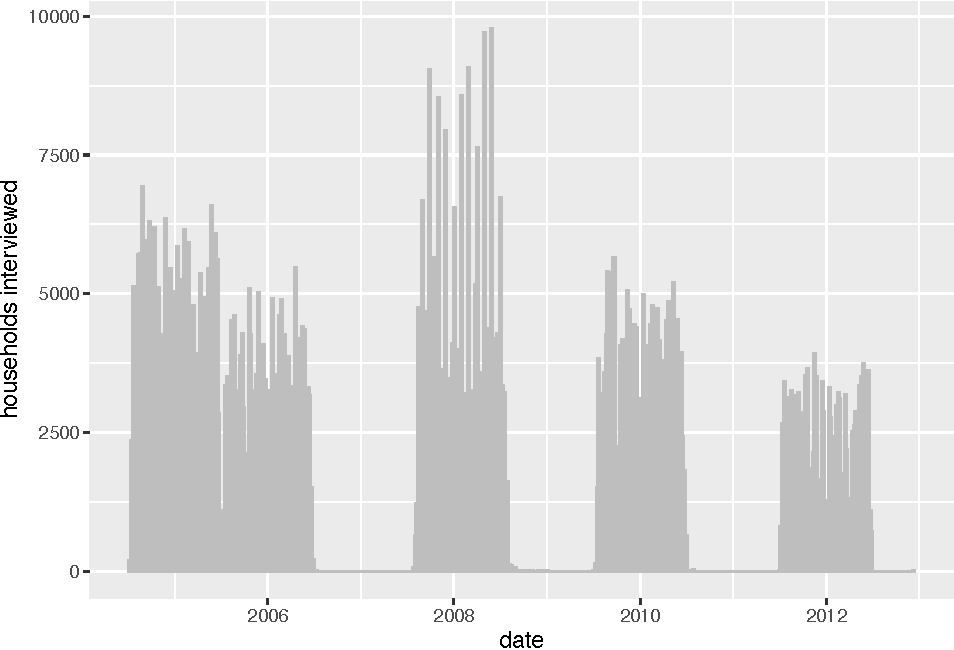
\includegraphics{draft_files/figure-latex/laborplot-1} \caption[Timing of household surveys for the National Sample Survey]{Timing of household surveys for the National Sample Survey}\label{fig:laborplot}\floatfoot*{Note: The histogram shows the distribution of survey dates for the four waves of the National Sample Survey (NSS) for the five waves used in this paper.}
\end{figure}

\FloatBarrier
\newpage
\begin{table}

\caption{\label{tab:labortablemonsoon}Wind direction and labor allocation, monsoon season only}
\centering
\begin{threeparttable}
\begin{tabular}[t]{>{\raggedright\arraybackslash}p{3cm}>{\centering\arraybackslash}p{1.5cm}>{\centering\arraybackslash}p{1.5cm}>{\centering\arraybackslash}p{1.5cm}>{\centering\arraybackslash}p{1.5cm}>{\centering\arraybackslash}p{1.5cm}>{\centering\arraybackslash}p{1.5cm}}
\toprule
  & all & all & self & wage & farm & non-farm\\
\midrule
wind & -0.021 & -0.033 & 0.038 & -0.071** & 0.072** & -0.105**\\
 & (0.028) & (0.029) & (0.034) & (0.033) & (0.036) & (0.046)\\
controls & No & Yes & Yes & Yes & Yes & Yes\\
\textbf{fixed effects:} & \textbf{} & \textbf{} & \textbf{} & \textbf{} & \textbf{} & \textbf{}\\
district & Yes & Yes & Yes & Yes & Yes & Yes\\
year & Yes & Yes & Yes & Yes & Yes & Yes\\
\textbf{varying slopes:} & \textbf{} & \textbf{} & \textbf{} & \textbf{} & \textbf{} & \textbf{}\\
year (by district) & Yes & Yes & Yes & Yes & Yes & Yes\\
\midrule
observations & 359,652 & 359,576 & 359,576 & 359,576 & 359,576 & 359,576\\
\bottomrule
\end{tabular}
\begin{tablenotes}
\item Note: Standard errors are in parentheses and are clustered at the district level. Control variables include female, age, age squared, and (years of) education.
\item * p<0.10 ** p<0.05 *** p<0.01
\end{tablenotes}
\end{threeparttable}
\end{table}

\FloatBarrier
\newpage
\begin{table}

\caption{\label{tab:labortablewinter}Wind direction and labor allocation, winter season only}
\centering
\begin{threeparttable}
\begin{tabular}[t]{>{\raggedright\arraybackslash}p{3cm}>{\centering\arraybackslash}p{1.5cm}>{\centering\arraybackslash}p{1.5cm}>{\centering\arraybackslash}p{1.5cm}>{\centering\arraybackslash}p{1.5cm}>{\centering\arraybackslash}p{1.5cm}>{\centering\arraybackslash}p{1.5cm}}
\toprule
  & all & all & self & wage & farm & non-farm\\
\midrule
wind & 0.003 & 0.002 & 0.011 & -0.009 & 0.024 & -0.022\\
 & (0.029) & (0.026) & (0.028) & (0.025) & (0.034) & (0.039)\\
controls & No & Yes & Yes & Yes & Yes & Yes\\
\textbf{fixed effects:} & \textbf{} & \textbf{} & \textbf{} & \textbf{} & \textbf{} & \textbf{}\\
district & Yes & Yes & Yes & Yes & Yes & Yes\\
year & Yes & Yes & Yes & Yes & Yes & Yes\\
\textbf{varying slopes:} & \textbf{} & \textbf{} & \textbf{} & \textbf{} & \textbf{} & \textbf{}\\
year (by district) & Yes & Yes & Yes & Yes & Yes & Yes\\
\midrule
observations & 375,956 & 375,883 & 375,883 & 375,883 & 375,883 & 375,883\\
\bottomrule
\end{tabular}
\begin{tablenotes}
\item Note: Standard errors are in parentheses and are clustered at the district level. Control variables include female, age, age squared, and (years of) education.
\item * p<0.10 ** p<0.05 *** p<0.01
\end{tablenotes}
\end{threeparttable}
\end{table}

\end{document}
